\normaltrue
\correctionfalse

%\UPSTIidClasse{11} % 11 sup, 12 spé
%\newcommand{\UPSTIidClasse}{12}

\exer{Mouvement RTR  $\star$ \label{DYN:04:1025}}
\setcounter{question}{0}\marginnote{\xpComp{DYN}{04}}%\xpComp{CIN}{02}%\UPSTIcompetence[2]{C2-05}


\index{Compétence DYN-04}

\ifcorrection
\else
\marginnote{\textbf{Pas de corrigé pour cet exercice.}}
\fi

\ifprof
\else

Soit le mécanisme suivant. On a $\vect{AB}=R\vect{i_1}$ et $\vect{BC}=\lambda(t)\vect{i_2}+r\vj{2}$. Le solide 1 est de masse $m_1$ et le plan $\left(A,\vect{i_1},\vect{j_1}\right)$ est plan de symétrie. Le solide 2 est de masse $m_2$ est axisymétrique d'axe $\axe{B}{i_2}$. On note $D$ son centre d'inertie.


On a :
\begin{itemize}
\item $G_1=B$ désigne le centre d'inertie de \textbf{1}, on note $m_1$ la masse de \textbf{1} et $\inertie{G_1}{1}=\matinertie{A_1}{B_1}{C_1}{0}{0}{0}{\bas{1}}$; 
\item $G_2=D$ désigne le centre d'inertie de \textbf{2} tel que  $\vect{BD}=\lambda\vect{i_2}$, on note $m_2$ la masse de \textbf{2} et $\inertie{G_2}{2}=\matinertie{A_2}{B_2}{C_2}{0}{0}{0}{\bas{2}}$.
\end{itemize}

\begin{figure}[H]
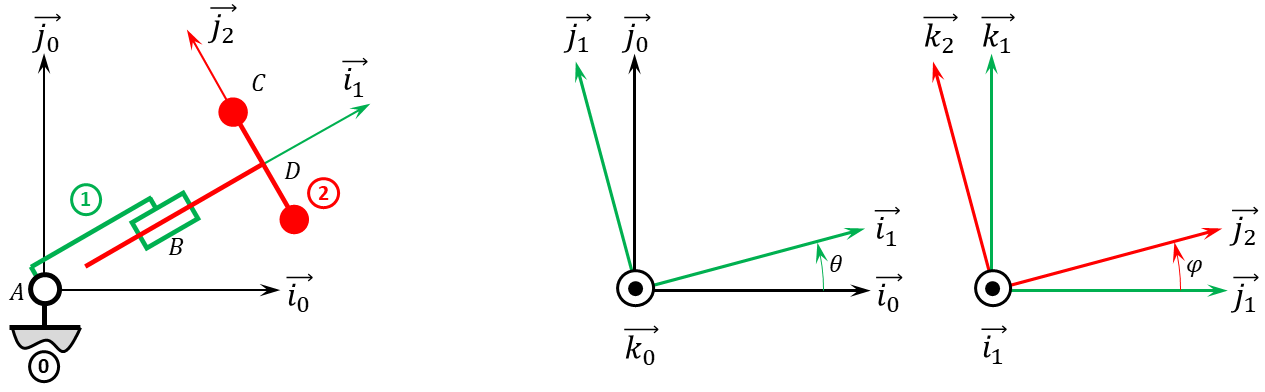
\includegraphics[width=\linewidth]{1025_01}
\end{figure}
\fi

\question{Déterminer $\vectrd{2}{0}\cdot\vect{i_1}$.}
\ifprof~\\
\else
\fi

\question{Déterminer $\vectmd{D}{2}{0}\cdot\vect{i_1}$.}
\ifprof~\\
\else
\fi

\question{Déterminer $\vectmd{A}{1+2}{0}\cdot\vect{k_0}$.}
\ifprof~\\
\else
\fi

\ifcolle
\question{Déterminer les lois du mouvement.}
\ifprof~\\
\else
\fi
\else
\fi

\ifprof
\else
\marginnote{Corrigé  voir \ref{DYN:04:1025}.}
\fi